\subsection*{Background}
A framed flow category $\fC$ is a collection of objects $\ob(\fC)$ with a grading function $\norm{-} : \ob(\fC) \to \bbZ$ and, for each pair of objects $y,x$ a moduli spaces between them $\flowM(y,x)$. In this paper we will assume that the moduli spaces are manifolds with corners, with tangential structure $\cX$ (e.g. a framing). Moreover, then are maps 
\[
    \flowM(z,y) \times \flowM(y,x) \hookrightarrow \flowM(z,x)
\]
which we think as gluing moduli spaces and the tangential structure is compatible with this gluing. The main example of a framed flow category is given by a Morse-Smale function on a closed manifold $\Man$, where the objects are the critical points, the grading is given by the index, and the moduli spaces are given by the compactified flow manifolds of $-\nabla f$. In this case the tangent structure is given by the stable framing of the flow manifolds.

The origins of framed flow categories can be traced back to the work of Cohen-Jones-Segal (CJS) in \cite{CJS95}. They showed that one can use Thom-Pontryagin construction (see \cite{thom1954quelques,pontryagin1955smooth}) to collapse a framed flow category into a stable homotopy type, a construction that generalized Morse chain complex and homology in two ways. First we can read off not only the homology of $M$ but also its stable homotopy type. Second, in many Floer-type theories the homology extracted from the geometry of a manifold $M$ is not the homology of $M$ nor the homology of a related manifold. This contusion allow us to realize a stable homotopy type from the geometry of $M$ even in cases where we cannot recover the homology of $M$.
 This framework has proven useful in other Floer-Type theories, where the solutions to the moduli problem sometimes exhibit the structure of a flow category $\fC$ \cite{chanda2025contact, }. Realizing $\fC$ and using stable homotopy tools led to breakthroughs in symplectic geometry, such as the proof of the Arnold conjecture over a field of characteristic $p$ (see \cite{abouzaid2021arnold}) and the integral Arnold conjecture (see \cite{rezchikov2022integral, bai2022arnold}) and other developments in Knot theory (see \cite{lipshitz2014steenrod}) and Lagrangian Floer theory (see \cite{abouzaid2018simple,porcelli2024bordism, porcelli2024spectral}).
 Another perspective on flow categories is given by the work of Abouzaid-Manolescu in \cite{abouzaid2024foundation}, where they define the stable $\infty$-category of framed flow categories and show that it is equivalent to the category of spectra.

\subsection*{Notations}
We denote by $\Top$ the $1$-category of topological spaces, by $\Spaces$ the category of homotopy types (or $\infty$-groupoids), and $\Sp$ is the category of spectra. The stabilization functor is denoted $\Sinf: \Spaces \to \Sp$, and $\Ch(\Sp)$ and $\Fil(\Sp)$ denote the categories of coherent chain complexes in Spectra and (complete) filtered Spectra, respectively.

For a topological space $Y$, we denote by $Y_+$ its one-point compactification (if $Y$ is compact, then $Y_+ = Y \cup \{*\}$).
For a CW complex $Y$, we denote by $\sk_n Y$ its $n$-th skeleton.

For a stable tangential structure $\xi: \cX \to BO$, we denote by $\Omega^{\cX}_*$ the graded $\cX$-bordism ring and by $M\cX$ the Thom spectrum associated with the $\cX$-structure (see \cref{sec:tangStr} for definitions).

In this paper, a manifold is assumed to be a \emph{closed manifold} unless stated otherwise.

 Let $\cX$ be a stable tangential structure, denote by $M\cX$ it's Thom spectrum. Given an $\cX$ flow category $\fC$, it is shown in \cite{Cohen19} that the realization $\norm{\fC}$ have a structure of an $M\cX$-module. Given a generalized homology $A \in \Sp$ with a map $A \to M\cX$ we define 
 \[
    A_*(\norm{\fC}) \coloneqq \pi_n(A \otimes_{M\cX} \norm{\fC}).
 \]

 Let $\fC$ be a flow category. For $q,p \in \bbZ$ we denote by $\fC_{[q,p]}$ the full subcategory of $\fC$ consisting of objects satisfying $q \ge \norm{x}\ge p$, and we define $\fC_p \coloneqq \fC_{[p,p]}$. For brevity, we write
\begin{equation*}
    M_{p,q}\coloneqq \bigsqcup_{y \in \fC_q, x \in \fC_p} M_{y,x}.
\end{equation*}

 Our first result is: 
 \begin{thm}
    Let $\fC$ be a flow category with an $\cX$-tangential structure and a spectrum $A$ over $M\cX$. There is a spectral sequence $\{E_r,d_r\}$ such that
    \begin{equation*}
        E_r \implies A_n(\norm{\fC}),
    \end{equation*}
    with first page given by
    \begin{equation*}
        E_1^{n,p} = \bigoplus_{\fC_p} A_{n-p}(\mathrm{pt}) = \bigoplus_{\fC_p} \pi_{n-p}(A).
    \end{equation*}
 \end{thm}

 If $A$ is bordism theory we have the following:
 \begin{thm}
    Let $\fC$ be a flow category with an $\cX$-tangential structure. Let $A = M\xi$ be the Thom spectrum which represents $\xi$ structured bordism homology, with a map of ring spectra $M\xi \to M\cX$.
    The spectral sequence of $\fC$ is given by
    \begin{equation*}
        E_1^{n,p} = \bigoplus_{\fC_p} \Omega^{\xi}_{n-p}.
    \end{equation*}
    Moreover, an element ...................
 \end{thm}

\subsection*{Our results}
\begin{defn}\label{def:Xrnp-extension}
Let $\fC$ be a flow category, and let $n, p, r \in \bbN$. Let $X = \{X_z\} \in \bigoplus_{z \in \fC_p} \Omega^{\operatorname{\cX}}_{n - p}$ be represented as a disjoint union of manifolds.

A \textbf{$(X,r,n,p)$-extension} of $\fC$ is a flow category $\fC'$ that satisfies:
\begin{equation*}
    \ob(\fC') = \fC_{[p,p-r]} \sqcup \{x\},\quad \norm{x}-p-1 = n-p
\end{equation*}
such that the flow manifolds of $\fC'$, denoted by $X_{a,b}$, satisfies:
\begin{equation*}
    X_{x, z} \simeq X_z,
\end{equation*}
and
\begin{equation*}
    X_{y,v} \simeq \flowM_{y,v}
\end{equation*}
for any $y,v \in \fC_{[p,p-r]}$ and $z \in \fC_p$.
\end{defn}
% survives to the r-th page iff r-1 extends
\begin{defn}\label{def:smallToda}
    Let $\fC'$ be a $(X,r,n,p)$-extension of $\fC$ and $y \in \fC_{p-(r+1)}$. We can define the punctured cube diagram:
    \begin{equation*}
        D_y: \ P(\{p,\dots,p-r\}) \setminus \{\varnothing\} \to \Top
    \end{equation*}
    where $P(-)$ is the power set, by setting
    \begin{equation*}
        D_y(\{a_k, \dots, a_1\}) = X_{x,a_k} \times M_{a_k,a_{k-1}} \dots \times M_{a_2,a_1} \times M_{a_1,y},
    \end{equation*}
    where $a_k > a_{k-1} > \dots > a_1$.
    
    The \textbf{Toda manifold} is the colimit
    \begin{equation*}
        \colim D_y
    \end{equation*}
\end{defn}
We will see later that the Toda manifolds indeed have a manifold structure, and that they are closed, $(n-p+r)$-dimensional, and $\cX$-structured.


\begin{exmp*}
    In \cref{fig:ffCat}, \ref{fig:k-boundary}, and \ref{fig:differential}, we can see an example of an extension and its Toda manifold.
\end{exmp*}

\begin{figure}[h!]
\[
% https://q.uiver.app/#q=WzAsNSxbMCwwLCJcXGJ1bGxldCJdLFswLDEsInhfMyJdLFswLDIsInhfMiJdLFswLDMsInhfMSJdLFswLDQsInhfMCJdLFswLDEsIk49IC0gXFwgLSIsMSx7ImxhYmVsX3Bvc2l0aW9uIjo4MCwic3R5bGUiOnsiYm9keSI6eyJuYW1lIjoibm9uZSJ9LCJoZWFkIjp7Im5hbWUiOiJub25lIn19fV0sWzEsMiwiTV97MywyfSA9ICtcXCArIiwxLHsic3R5bGUiOnsiYm9keSI6eyJuYW1lIjoibm9uZSJ9LCJoZWFkIjp7Im5hbWUiOiJub25lIn19fV0sWzIsMywiTV97MiwxfSA9ICtcXCAtIiwxLHsibGFiZWxfcG9zaXRpb24iOjIwLCJzdHlsZSI6eyJib2R5Ijp7Im5hbWUiOiJub25lIn0sImhlYWQiOnsibmFtZSI6Im5vbmUifX19XSxbMyw0LCJNX3sxLDB9ID0gKyIsMSx7ImxhYmVsX3Bvc2l0aW9uIjoyMCwic3R5bGUiOnsiYm9keSI6eyJuYW1lIjoibm9uZSJ9LCJoZWFkIjp7Im5hbWUiOiJub25lIn19fV0sWzIsNCwiSSIsMSx7ImN1cnZlIjotNX1dLFsxLDMsIkkgXFwgSSIsMSx7ImN1cnZlIjo0fV0sWzAsMiwiSSBcXCBJIiwxLHsiY3VydmUiOi01fV0sWzEsNCwiSV4yIiwxLHsiY3VydmUiOjUsImxldmVsIjoyfV0sWzAsMywiSV4yIiwxLHsiY3VydmUiOi01LCJsZXZlbCI6Mn1dXQ==
\begin{tikzcd}[column sep=huge]
    x & {x_4} & {x_3} & {x_2} & {x_1}
    \arrow["{X= - \sqcup -}"'{yshift=-5pt},curve={height=-10pt}, from=1-1, to=1-2, thick, dashed]
    \arrow["{X_{5,3}=I \sqcup I}"{description}, curve={height=30pt}, from=1-1, to=1-3, color=myred, dashed]
    %\arrow["{X_{5,2}=I^2}"{description}, curve={height=60pt}, Rightarrow, from=1-1, to=1-4, color=myblue, dashed]
    \arrow["{X_{5,2}=I^2}"{description}, curve={height=60pt}, from=1-1, to=1-4, color=myblue, dashed]
    \arrow["M_{4,2}={I \sqcup I}"'{description}, curve={height=-30pt}, from=1-2, to=1-4, color=mygreen]
    \arrow["M_{3,1}=I"{description}, curve={height=-30pt}, from=1-3, to=1-5, color=myyellow,crossing over]
    %\arrow["{M_{4,1}=I^2}"{description}, curve={height=-60pt}, Rightarrow, from=1-2, to=1-5, color=myviolet]
    \arrow["{M_{4,1}=I^2}"{description}, curve={height=-60pt}, from=1-2, to=1-5, color=myviolet]
    \arrow["{M_{4,3} = - \sqcup +}"'{yshift=-5pt},curve={height=-10pt}, from=1-2, to=1-3]
    \arrow["{M_{3,2} = + \sqcup -}"'{yshift=-5pt},curve={height=-10pt}, from=1-3, to=1-4]
    \arrow["{M_{2,1} = +}"'{yshift=-5pt},curve={height=-10pt}, from=1-4, to=1-5]
\end{tikzcd}
\]
\caption{
The solid part represents the flow category $\fC$. Its objects are the $x_i$'s with $\norm{x_i}=i$, and the arrows represent the morphism manifolds.
The 0 dimensional framed manifold $X$ represents an element in $E_1^{4,4} = \Omega^{\fr}_{4-4}$.
The dashed arrows represent an $(X,2,4,4)$-extension.
Note that the whole diagram does not represent a flow category, as $X_{5,1}$ is missing.
The symbols $\pm$, $I$, etc., represent the flow manifolds themselves (where $\pm$ represents a framed point; the rest of framing is omitted for clarity).
}\label{fig:ffCat}
\end{figure}

\captionsetup{font={small}}
\begin{figure}[h!]
\centering
\begin{minipage}{.61\textwidth}
  \centering
  \adjustbox{width=\linewidth}{\begin{tikzcd}
{X\times M_{4,3}\times M_{3,2}\times M_{2,1}} && |[myyellow]|{X\times M_{4,3}\times M_{3,1}}& \\
\\
& |[mygreen]|{X\times M_{4,2}\times M_{2,1}} && |[myviolet]|{X\times M_{4,1}} \\
\\
|[myred]|{X_{5,3}\times M_{3,2}\times M_{2,1}} && |[orange]|{X_{5,3} \times M_{3,1}} \\
\\
& |[myblue]|{X_{5,2}\times M_{2,1}}
\arrow[gray,from=1-1, to=1-3]
\arrow[gray,from=1-1, to=3-2]
\arrow[gray,from=1-1, to=5-1]
\arrow[gray,from=1-3, to=3-4]
\arrow[gray,from=1-3, to=5-3]
\arrow[gray,from=5-1, to=5-3]
\arrow[gray,from=5-1, to=7-2]
\arrow[gray,from=3-2, to=7-2, crossing over]
\arrow[gray,from=3-2, to=3-4, crossing over]
\end{tikzcd}}
  \captionof{figure}{
  The extension of \cref{fig:ffCat} (from $x$ to $x_2$) and the\\object $x_1$ construct the punctured cube $D_{x_1}$
  }
  \label{fig:k-boundary}
\end{minipage}\hfill
\begin{minipage}{.37\textwidth}
  \centering
  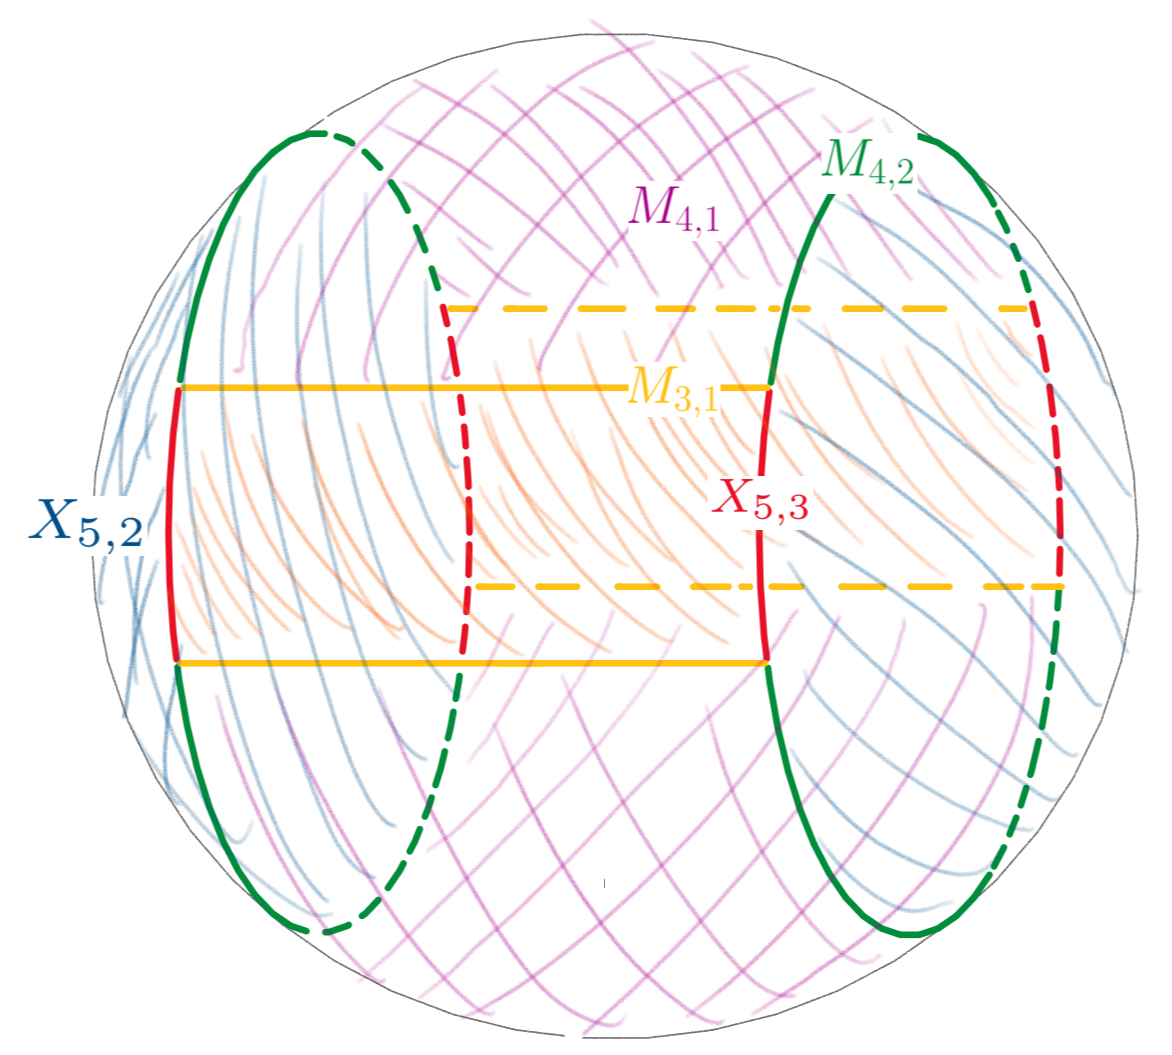
\includegraphics[width=\linewidth]{fig/differential.png}
  \captionof{figure}{
  We can see that $\colim D_{x_1}$ is a topological space that inherits a closed smooth manifold structure.
  }
  \label{fig:differential}
\end{minipage}
\end{figure}
%\newpage
\begin{restatable}{thmA}{ThA}\label{SSofStrFFCat}
    Let $\fC$ be a flow category with an $\cX$-tangential structure. There is a spectral sequence:
    \begin{equation*}
        \pg{E}{1}{n}{p} = \bigoplus_{\norm{z}=p} \Omega^{\cX}_{n-p}
    \end{equation*}
    which converges to the homotopy groups of the realization:
    \begin{equation*}
        \rnp{E} \implies \pi_n \norm{\fC}.
    \end{equation*}
    An element $X_z \in \pg{E}{1}{n}{p}$ survives to $\pg{E}{r+1}{n}{p}$ if and only if there exists an $(X,r,n,p)$ extension of $\fC$. Let $\fC'$ be such an extension. The differential is represented geometrically by the Toda manifolds:
    \begin{equation*}
        d_{r+1}(X) = \bigsqcup_{y \in \fC_{p-(r+1)}} \colim D_y
    \end{equation*}\todo{write as $\bigcup$}
    viewed as an element
    \begin{equation*}
        d_{r+1}(X) \in \bigoplus_{y \in \fC_{p-(r+1)}} \Omega^{\cX}_{n-p+r} = \pg{E}{r+1}{n-1}{p-(r+1)}.
    \end{equation*}
\end{restatable}
We interpret the existence of an $(r,n,p)$-extension of $X$ as the condition $X \in \ker\ d_r$.

A key tool used to prove \cref{SSofStrFFCat} is a description of the spectral sequence associated with a coherent chain complex expressed in terms of chain complex maps.

\begin{restatable}{thmA}{ThB}\label{SSofCh}
    Let $K \in \Ch(\Sp)$ be a coherent chain complex in Spectra. Then there is a spectral sequence:
    \begin{equation*}
        E_1^{n,p} = \pi_{n - p} K_p,
    \end{equation*}
    which converges to
    \begin{equation*}
        E_r^{n,p} \implies \pi_n \colim_p (\cI K)_p,
    \end{equation*}
    
    Moreover, let $x: \mathbb{S}^{n - p} \to K_p$ represent an element of $\pg{E}{1}{n}{p}$. Then $x$ survives to $\pg{E}{r+1}{n}{p}$ if and only if there exists a chain map:
    \begin{equation}\label{eq:x_ext}
        \xymatrix{
        \mathbb{S}^{n - p} \ar[d]_{x} \ar[r] & 0 \ar[r]\ar[d] & \dots \ar[r]\ar[d]& 0\ar[d]\\
        K_p \ar[r]^{d_p}& K_{p - 1} \ar[r]^{d_{p - 1}}& \dots \ar[r]^{d_{p - r} \quad}& K_{p - r}
        }
    \end{equation}
    Here, the top row is concentrated in degree $p$, and the bottom row is the restriction of $K$ from degree $p$ down to $p-r$.
    The differential $\partial_{r+1}(x)$ is given by the composition of chain maps:
    \begin{equation*}
        \xymatrix
        {   \mathbb{S}^{n-p} \ar[r]\ar[d]_x & \dots \ar[r]\ar[d] &  0 \ar[d]\\
            K_p \ar[r]\ar[d] & \dots \ar[r]\ar[d] &  K_{p-r} \ar[d] \\
            0 \ar[r] & \dots \ar[r] & K_{p-r-1} 
        }
    \end{equation*}
    The first map is precisely \cref{eq:x_ext} and the second is induced by the structure of the chain complex $K$.
\end{restatable}
We obtain this result by combining the description of the spectral sequence of a filtered object in Lurie \cite{Lur17} with the results of~\cite{Ari21}.

\subsection*{Relation to other work}\todo{Delete everything which is not directly related to flow categories (delete all the Khovanov, Arnold, knots,...)}
This paper contributes to the broader project of providing a geometric model for spectra. For the foundation of this project, which defines the stable $\infty$-category of framed flow categories and establishes its equivalence with the category of spectra, see \cite{abouzaid2024foundation}.

This project traces back to the work of Cohen–Jones–Segal (CJS) in \cite{CJS95}, where the term “flow category” was introduced as a means of organizing the data of a Morse–Smale function in a categorical way. In that work, a coherent version of chain complexes is constructed from such a category, and these chains are subsequently “realized” as a filtered spectrum. These ideas have since proven very useful in Floer theory.

In knot theory, organizing the data of knots into a flow category results in a stable homotopy type that lifts Khovanov homology (see \cite{LS14}). Moreover, by simplifying the flow categories (see \cite{lobb2018framed, lobb2017calculus}) and classifying $0$- and $1$-dimensional manifolds, one obtains a combinatorial description and an effective algorithm for computing the operations
\[
    \operatorname{Sq}^2 : H^\ast(\fC, \mathbb{Z}/2) \to H^{\ast+2}(\fC, \mathbb{Z}/2)
\]
from a knot diagram. This leads to the calculation of the corresponding homotopy (see \cite{lobb2020khovanov, lipshitz2014steenrod}). For a recap of flow categories in Khovanov and knot Floer theories, see \cite{marengon2024spectra}.

Our work is similar in spirit to these developments in that we use higher flow manifolds to compute the differentials, which can be interpreted as higher cohomology operations.

In Hamiltonian Floer theory, one of the breakthroughs related to the Arnold conjecture employed a CJS-like construction—a generalization of flow categories adapted to Hamiltonian flow data—to prove a version of the Arnold conjecture over a field of characteristic $p$ (see \cite{abouzaid2021arnold}). Similar ideas appear in the work on the integral Arnold conjecture (see \cite{rezchikov2022integral, bai2022arnold}). Another recent development is the theory of Morse–Bott flow categories, where the function has critical sets (rather than isolated points) (see \cite{bonciocat2024revisiting}). An ongoing line of research is the introduction of an equivariant structure on such categories, which in turn induces an equivariant structure on the realization spectrum—a framework that supports cyclotomic methods in symplectic geometry (see \cite{cote2023equivariant, rezchikov2024cyclotomic}).

One also finds flow-category–like constructions in Lagrangian geometry that lift the Fukaya category of a symplectic manifold (see \cite{porcelli2024bordism, porcelli2024spectral}).

\begin{rem}
    In this paper we treat flow categories as chain complexes in $\Sp$ or, equivalently, as filtered spectra. We expect that there is a construction analogous to that in \cite{abouzaid2024foundation} which provides a flow-categorical model for $\{K_p\} \in \Ch(\Sp)$ such that $K_p = \bigoplus \mathbb{S}$.
\end{rem}

The interpretation of gluing manifolds as Toda brackets or Massey products appears in \cite{alexander1972cobordism}, where the Massey product is defined via the gluing of two manifolds with boundary.

\Cref{SSofCh} bears a similar flavor to other works on spectral sequences associated with various objects. In \cite{Ari21}, the authors explain the connection between filtered objects and coherent chain complexes, and they also define a spectral sequence for coherent chain complexes using the Beilinson $t$-structure. We also recommend \cite{antieau2024spectral} as an introduction to spectral sequences and their relation both to chain complexes and to the spectral sequence of filtered objects defined in \cite{Lur17}. The construction of the spectral sequence in this paper is similar to that in \cite{blanc2022spectral}, where the authors define a spectral sequence associated with a simplicial object.

\subsection*{Paper layout}
Section~2 is devoted to the framework of chain complexes in (stable) $\infty$-categories and contains the proof of \Cref{SSofCh}.

In Section~3, we recall the definitions of manifolds with corners, framed flow categories, and the Pontryagin–Thom construction for manifolds with corners. At the end of this section, we demonstrate several properties of the Pontryagin–Thom construction that will be useful in later sections.

Section~4 establishes a correspondence between chain complexes in the category of spectra (with values $\bigoplus \mathbb{S}$) and framed flow categories.

Our goal in Sections~5 and~6 is to upgrade this correspondence so that it interacts naturally with spectral sequences. In other words, given a framed flow category, we show how to produce a spectral sequence for the corresponding chain complex and provide a geometrical description of its pages and differentials.

In Section~5, we compare various models for chain complexes by considering different models for $\infty$-categories (namely, topologically enriched, simplicially enriched, and simplicial sets). This comparison allows us to give a straightforward description of the composition of maps between flow categories.

Section~6 translates this description of composition into a geometrical framework and establishes the existence of a spectral sequence associated with framed flow categories.

In the final section, we explain how the framing structure can be replaced by a more general tangential structure, and we discuss how different structures interact. This section also contains examples of spectral sequences arising from flow categories.

\subsection*{Discussion and open problems}
\textbf{Different definitions for flow categories.} In \cite{abouzaid2024foundation}, the authors construct an $\infty$-category $\mathrm{Flow}^{\fr}$ (see also \cite{porcelli2024bordism} for the homotopy category) and show that it is equivalent to $\Sp$. We now explain the main difference between their work and ours from an algebro-topological perspective. Let $M$ be a compact manifold. Given two Morse–Smale functions $f$ and $g$, one obtains two framed flow categories, $\fC_f$ and $\fC_g$. By interpolating between $f$ and $g$, we obtain two maps in $\mathrm{Flow}^{\fr}$
\[
    H_{f,g}: \fC_f \to \fC_g, \quad H_{g,f}: \fC_g \to \fC_f,
\]
and by homotoping the compositions we obtain 2-morphisms
\[
    H_{g,f} \circ H_{f,g} \simeq \mathrm{Id}, \quad H_{f,g} \circ H_{g,f} \simeq \mathrm{Id}.
\]
Hence, the flow category of $M$ is independent of the choice of Morse–Smale function.

On the other hand, the functions $f$ and $g$ induce CW structures on $M$, and different CW structures yield different (Atiyah–Hirzebruch) spectral sequences. Therefore, one cannot define a spectral sequence as an invariant of the equivalence classes in $\mathrm{Flow}^{\fr}$.

To address this issue, we conjecture that one can define another $\infty$-category, with a modified class of morphisms. Specifically, for a 2-morphism $R$ between flow categories $\fC$ and $\sD$, and for objects $x \in \fC$ and $y \in \sD$, we require that if $\|y\| > \|x\|$, then $R_{x,y} = \varnothing$ (rather than being a manifold of dimension $\|y\| - \|x\|$). This construction should yield a subcategory of $\Fil(\Sp)$ in which the two Morse–Smale functions on a manifold $M$ produce distinct objects.

Using this perspective, we can think of \cref{SSofStrFFCat} as a spectral sequence of filtered flow category $F \in \Fil(\mathrm{Flow}^{\cX})$ where the filtration is induces by the index filtration on a flow category.

In this paper the full $\infty$-categorical structure is unnecessary; instead, we define the equivalence relation on flow categories by pulling it back from the category $\Ch(\Sp)$ (see \Cref{prop:FF_are_Ch}).